\documentclass[a4paper,10pt]{article}
\usepackage{fullpage}
\usepackage[british]{babel}
\usepackage[T1]{fontenc}
\usepackage{amsmath}
\usepackage{amssymb}
\usepackage[T1]{fontenc}
\usepackage[utf8]{inputenc}
%\usepackage{amsthm} \newtheorem{theorem}{Theorem}
\usepackage{color}


\usepackage{float}
\usepackage{enumerate}
\usepackage{caption}
\DeclareCaptionFont{white}{\color{white}}
\DeclareCaptionFormat{listing}{\colorbox{gray}{\parbox{\textwidth}{#1#2#3}}}
\captionsetup[lstlisting]{format=listing,labelfont=white,textfont=white}

\usepackage{alltt}
\usepackage{listings}
 \usepackage{aeguill}
\usepackage{dsfont}
%\usepackage{algorithm}
\usepackage[noend]{algorithm2e}
%\usepackage{algorithmicx}
\usepackage{subfig}
\lstset{% parameters for all code listings
language=Python,
frame=single,
basicstyle=\small, % nothing smaller than \footnotesize, please
tabsize=2,
numbers=left,
% framexleftmargin=2em, % extend frame to include line numbers
%xrightmargin=2em, % extra space to fit 79 characters
breaklines=true,
breakatwhitespace=true,
prebreak={/},
captionpos=b,
columns=fullflexible,
escapeinside={\#*}{\^^M}
}


% Alter some LaTeX defaults for better treatment of figures:
    % See p.105 of "TeX Unbound" for suggested values.
    % See pp. 199-200 of Lamport's "LaTeX" book for details.
    % General parameters, for ALL pages:
    \renewcommand{\topfraction}{0.9}	% max fraction of floats at top
    \renewcommand{\bottomfraction}{0.8}	% max fraction of floats at bottom
    % Parameters for TEXT pages (not float pages):
    \setcounter{topnumber}{2}
    \setcounter{bottomnumber}{2}
    \setcounter{totalnumber}{4} % 2 may work better
    \setcounter{dbltopnumber}{2} % for 2-column pages
    \renewcommand{\dbltopfraction}{0.9}	% fit big float above 2-col. text
    \renewcommand{\textfraction}{0.07}	% allow minimal text w. figs
    % Parameters for FLOAT pages (not text pages):
    \renewcommand{\floatpagefraction}{0.7}	% require fuller float pages
% N.B.: floatpagefraction MUST be less than topfraction !!
    \renewcommand{\dblfloatpagefraction}{0.7}	% require fuller float pages

% remember to use [htp] or [htpb] for placement


\usepackage{fancyvrb}
%\DefineVerbatimEnvironment{code}{Verbatim}{fontsize=\small}
%\DefineVerbatimEnvironment{example}{Verbatim}{fontsize=\small}

\usepackage{url}
\urldef{\mailsa}\path|josh0151@student.uu.se |
\urldef{\mailsb}\path|bjfo5755@student.uu.se |
\newcommand{\keywords}[1]{\par\addvspace\baselineskip
\noindent\keywordname\enspace\ignorespaces#1}


\usepackage{tikz} \usetikzlibrary{trees}
\usepackage{hyperref} % should always be the last package

% useful colours (use sparingly!):
\newcommand{\blue}[1]{{\color{blue}#1}}
\newcommand{\green}[1]{{\color{green}#1}}
\newcommand{\red}[1]{{\color{red}#1}}

% useful wrappers for algorithmic/Python notation:
\newcommand{\length}[1]{\text{len}(#1)}
\newcommand{\twodots}{\mathinn\usepackage{enumerate}er{\ldotp\ldotp}} % taken from clrscode3e.sty
\newcommand{\Oh}[1]{\mathcal{O}\left(#1\right)}

% useful (wrappers for) math symbols:
\newcommand{\Cardinality}[1]{\left\lvert#1\right\rvert}
%\newcommand{\Cardinality}[1]{\##1}
\newcommand{\Ceiling}[1]{\left\lceil#1\right\rceil}
\newcommand{\Floor}[1]{\left\lfloor#1\right\rfloor}
\newcommand{\Iff}{\Leftrightarrow}
\newcommand{\Implies}{\Rightarrow}
\newcommand{\Intersect}{\cap}
\newcommand{\Sequence}[1]{\left[#1\right]}
\newcommand{\Set}[1]{\left\{#1\right\}}
\newcommand{\SetComp}[2]{\Set{#1\SuchThat#2}}
\newcommand{\SuchThat}{\mid}
\newcommand{\Tuple}[1]{\langle#1\rangle}
\newcommand{\Union}{\cup}
\usetikzlibrary{positioning,shapes,shadows,arrows}

\usepackage{url}

\pagestyle{empty}

\title{\textbf{The History, Development and Future of \\
	Computer Input/Output devices}}

\author{Bj{\"o}rn Forsberg, Jonathan Sharyari}
\oddsidemargin 0.5in 
\textwidth 5.5in 
\begin{document}


\maketitle




\section{Introduction}
During the history of computers, many means of interaction with computers have been used. This frame of interaction is often important. For example, the lack of appropriate input/output devices may limit the use of the computer despite the technology and processing power being available. The lack of appropriate interfaces may also make computer use unnecessary complicated. In some ways, the input/output devices constitute the basis of interaction between users and computers, and dictates how software is developed in general. How would the desktop look, had it not been for the invention and popularisation of the computer mouse? 

Currently the development of mobile operating systems and mobile applications are growing rapidly - a development tightly linked to the differences in input/output methods. These changes have had a great impact on how we lead our life, by integrating computers to everyday tasks. Consider the simple example of someone taking the bus. Using a mobile device, she may first use it to check the bus time table, then purchase a bus ticket online and during the duration of the trip entertain herself by reading a book or listening to music.

As the role of computers in society has increased and infiltrated many aspects of every day life, it has become an important democratic issue that no group of people is systematically left outside of this development. This implies the need of a broad set of special-purpose devices aimed to aid people with specials needs, for example people with impaired vision, hearing or motor skills. 

These topics are just a subset of topics within the scope of this subject. To break it down, we propose to divide the project into four parts which raise questions of different nature.
\begin{enumerate}
\item
The history of input/output devices
\item
Current input/output devices, and the reasoning leading up to their creation and popularization
\item
Possible future input/output devices and what justifies them
\item
Special-purpose devices
\end{enumerate}

\section{Scope}

The scope of this project is to understand and analyse the history, the present and the future of computer input devices. The main focus is input devices, although output devices will be included as far as is needed. In some cases, for example, the input and output devices form a subsystem, where one would not work without the other. Examples of such subsystems are the computer mouse and its dependency of the bitmap computer screen, as well as the touchscreen that provides both input and output functionality. 

The input devices discussed in this paper are the input devices used with traditional computers, laptops and hand-held computers including smart phones and tablets. Cell phones, embedded systems, game stations and other computer-aided devices are not included.

The time frames in this project are divided into historical systems (-2000), present systems (2000-2013) and future systems (2013-). This is a rough and subjective categorization, and naturally some overlap is inevitable. Some devices that are seen as historical, such as the keyboard, are still in wide use today and will likely continue to be in the foreseeable future. But it is also possible that devices that are to be seen as future devices have already been developed but not popularised.

\section{Background}
Although input/output devices is a big subject, only a few articles discuss the history of computer input devices in depth\cite{aspray}\cite{myers}.  The articles that focus on input devices often focus on one device or device type, and a comparison between different implementations of that type\cite{facial}\cite{azenkot}\cite{prescher}.

We believe that the value of analysing the history underlying the development of input devices is worthwhile. An understanding of the processes that lead up to the devices we have today can broaden our understanding of the input device development process, which is the main knowledge gap that we aim to fill through this project.

The main search words used for finding previous research in the historic field are "Human Computer Interface", "Input device", "Input-output program", "Human Interface Device", "Input-output devices" and variations of these terms combined with search categories "history", "history of ideas", "overview" and variations thereof. The main search words for finding research about special purpose devices are "physically disabled", "physically challenged" and "motor skills", combined with the earlier categories; "human computer interaction", "human computer interface" and "computer peripheral equipment".

\section{Aims and Objectives}
\subsection{Aims}
\begin{itemize}
\item
Investigate which factors lead to the development of new interaction methods.
\item
Investigate the alternatives available for people that for some reason cannot use mainstream input/output devices.
\item
See if there are any common factors in the development of new input/output devices. Are they technology driven or user need driven?
\end{itemize}
\subsection{Objectives}
\begin{itemize}
\item
Present a summary of the history of the input/output devices.
\item
Describe the input/output devices that are under development now, their goals, their usage areas and the technology involved.
\item
A well-founded prediction of how future input/output devices will work.

\end{itemize}


\section{Question formulation}	

We have structured the questions in chronological order, as we believe it is important to understand the history of input devices to get a good understanding of what led to contemporary devices, and what might come next. This will hopefully aid us in continuously asking the right questions to understand the development of later technologies and the context in which they were introduced.

The same principle applies to the future devices that are in development now - in order to understand their development and goals we need to understand the current context and the perceived improvements the new devices offer.

The special purpose devices do not have the same chronological dependencies. Their context is more related to the input devices considered as standard at their point of introduction, as the computer interfaces are designed to work well for them. This means that to understand the special purpose devices, we have to look at the interface designs of the time, and what parts of the related interfaces that propose a problem to certain users, and how the device in question circumvents this problem.

\begin{enumerate}
	\item
	Past
	\begin{enumerate}[I]
		\item How did the first generation of input devices work?
		\item What is the background of the first "user friendly" input devices? How did this change occur?
	\end{enumerate}

	\item
	Current
	\begin{enumerate}[I]
		\item What are the backgrounds to today’s input devices (touchscreens, voice recognition)?
		\item What are the challenges set upon these devices?
		\item Optionally\footnote{If there is time available.}: What are the bigger "visions" about how computer interaction should work?
	\end{enumerate}

	\item
	Future
	\begin{enumerate}[I]
		\item What input devices are in the pipeline now?
		\item What are the target markets? Will they replace the current input methods, or will they change the computer 	interaction overall?
	\end{enumerate}

	\item
	Special-purpose devices
	\begin{enumerate}[I]
		\item
		What alternatives exist for the physically impaired?
		\item
		Optionally: How do these cope with the challenges set upon by those using them and by the broad range of uses computer applications in use today?
		\item
		How does the development currently proceed, and what importance is this issue perceived to have?
	\end{enumerate}
\end{enumerate}

\section{Methodology}
\label{sec:method}
We will use a Scrum-inspired\cite{scrum} method in this project, with one week \emph{sprints} during which we will do the work necessary to complete each part of the final report. The idea is to divide the work into a set of fairly independent blocks and that each sprint should result in a deliverable sub-report. These blocks will be integrated in a final stage as to avoid repetition and to improve the general flow of the report. We will also do some continuous integration to allow for cross-referencing.

The project will be divided into the following parts:
\begin{enumerate}
	\item \textbf{Special-purposed devices.} Gather information about which special-purpose methods have been used to overcome accessibility problems.
	\item \textbf{History.} Gather information about historical input/output methods (i.e. used before the year 2000), why they were successful or unsuccessful, how they were developed and how they affected the interaction with computers.
	\item \textbf{Contemporary devices.} Gather information about the input/output methods used between the years 2000 and up to now. Which methods were proposed, which were successful, how were they developed and how did they affect the interaction with computers.
	\item \textbf{Discussion/Analysis (text body).} Analysis of the development up until now. Are there any common factors? How has the thinking of the past led to the methods we used today, and are there any points where the development could have gone in another direction if they would have been done today? This will hopefully lead to a better understanding of the challenges of future devices.
	\item \textbf{Future devices.} Gather information about the directions the input/output methods are going in today. What concepts are in the pipeline, what are their goals and markets, and what changes would they bring to the way we use computers in the future?
	\item \textbf{Discussion/analysis (full report)}. Which conclusions can be drawn? This should concentrate mostly on the future devices, as this topic is only a prediction of what may or may not be in the future, but there is also reason to critically examine the results of historical devices.

\end{enumerate}

\section{Project plan and deliverables}
\paragraph{Deliverables}
This project is planned to result in a set of deliverables, beside the final report. This includes a \textbf{review} of a relevant reference paper, to be completed at an early stage of the project. A \textbf{poster} with the most general results, and a set of \textbf{slides} to aid a final presentation of the project. We will also deliver an \textbf{outline} of the report at an early stage, and a \textbf{preliminary report} at a later stage that is to be subject of external review.


\paragraph{Time plan}

The Gantt diagram in Figure 1 shows the preliminary time plan for the project. Each week is estimated to need twenty hours of work each, with the exception of week 16 when additional effort is needed in order to meet the deadlines on some of the deliverables, as well as completing the two initial sprints. In total, the project will need about 140 hours to complete.

The plan is to avoid working in parallell. Instead both participants work simultaniously, although not necessarily with the same topic. This encourages continuous discussion and better ensures that common ground has been reached on all topics in the report. Situations were one of the participants gets stuck on a topic can be avoided by continously switching work tasks, which also allows for better utilization of the strengths of the participants.

\begin{figure}[h!]
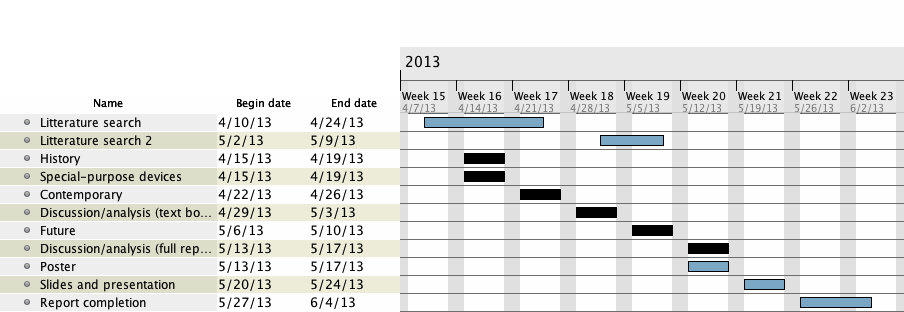
\includegraphics[width=\textwidth]{ganttuppsats.png}
\caption{Preliminary project plan. The boxes in black correspond to sprints as explained \hyperref[sec:method]{above}.}
\label{fig:timePlan}
\end{figure}


\begin{thebibliography}{4}
\bibitem{scrum} Schwaber, K. (2003). \emph{Agile Project Management with Scrum}. Redmond: Microsoft Press
\bibitem{aspray} W Aspray. \emph{Computers Before Computing}. Iowa State University Press, Ames, Iowa, 1990.
\bibitem{myers}B.A. Myers. \emph{A brief history of human-computer interaction technology}. Interactions, 5(2):44–54, 1998.
\bibitem{eniac}S. McCartney. \emph{ENIAC: the triumphs and tragedies of the world’s first computer}. Walker \& Company, 1999.
\bibitem{facial}K. Parmar, B. Mehta, and R. Sawant. \emph{Facial-feature based Human-Computer Interface for disabled people}. In Communication, Information Computing Technology (ICCICT), 2012 International Conference on, pages 1–5, 2012.
\bibitem{azenkot}
Shiri Azenkot, Jacob O. Wobbrock, Sanjana Prasain, and Richard E. Ladner. \emph{Input finger detection
for nonvisual touch screen text entry in Perkinput}. In Proceedings of Graphics Interface 2012, GI ’12,
pages 121–129, Toronto, Ont., Canada, Canada, 2012. Canadian Information Processing Society.
\bibitem{prescher}
Prescher, D., Weber, G. and Spindler, M. (2010). \emph{A Tactile Windowing System for Blind Users}. ASSETS’10, October 25–27, 2010, Orlando, Florida, USA.
\end{thebibliography}

\end{document}
